\documentclass[paper=a4, fontsize=11pt]{scrartcl}
\usepackage{fourier}
\usepackage[table,xcdraw]{xcolor}
\usepackage[protrusion=true,expansion=true]{microtype}	
\usepackage{amsmath,amsfonts,amsthm} % Math packages
\usepackage{graphicx}	
\usepackage{url}
\usepackage{bookmark}

\usepackage{polyglossia}
\setdefaultlanguage{greek}
\setotherlanguages{english}
%%% Bibliography 
\usepackage{biblatex}
\addbibresource{ref.bib}
\usepackage{float}
\restylefloat{table}
%%%% algorithms
\usepackage{algorithm} 
\usepackage{algpseudocode} 
\usepackage{enumitem}

\graphicspath{ {./images/} }


%%%fonts
\usepackage{fontspec}
\setmainfont{FreeSerif}
\setsansfont{FreeSans}
\setmonofont{FreeMono}


\usepackage{sectsty}
\allsectionsfont{\centering \normalfont\scshape}


%%% Custom headers/footers (fancyhdr package)
\usepackage{fancyhdr}
\pagestyle{fancyplain}
\fancyhead{}											% No page header
\fancyfoot[L]{}											% Empty 
\fancyfoot[C]{}											% Empty
\fancyfoot[R]{\thepage}									% Pagenumbering
\renewcommand{\headrulewidth}{0pt}			% Remove header underlines
\renewcommand{\footrulewidth}{0pt}				% Remove footer underlines
\setlength{\headheight}{13.6pt}


\numberwithin{equation}{section}		% Equationnumbering: section.eq#
\numberwithin{figure}{section}			% Figurenumbering: section.fig#
\numberwithin{table}{section}				% Tablenumbering: section.tab#

%%%paragraph 
\setlength{\parindent}{1em}
\setlength{\parskip}{0.5em}

\usepackage{titlesec, lipsum}
\titleformat{\paragraph}[block]{\filcenter}{}{0pt}{}

%%% Maketitle metadata
\newcommand{\horrule}[1]{\rule{\linewidth}{#1}}

\usepackage{lipsum}
\usepackage{fancyhdr}


\pagestyle{fancy}
\fancyhf{} % Εκκαθάριση όλων των ρυθμίσεων
\fancyhead[C]{Τμήμα Πληροφορικής \& Τηλεπικοινωνιών}
\fancyhead[R]{\includegraphics[width=1cm]{right.png}}
\fancyhead[L]{\includegraphics[width=1cm]{left.png}}

\fancyfoot[C]{Αλγόριθμοι & Προχωρημένες Δομές Δεδομένων
                \\Βίννη Παναγιώτα}

\fancyfoot[R]{\thepage}

\usepackage[colorlinks]{hyperref}
\usepackage{xcolor}
\usepackage{titlesec}

\title{
     \usefont{OT1}{bch}{b}{n}
     \normalfont \normalsize \textsc{Πανεπιστήμιο Ιωαννίνων Τμήμα Πληροφορικής \& Τηλεπικοινωνίων} \\ [1em]
     \normalfont \normalsize \textsc{Πρόγραμμα Μεταπτυχιακών Σπουδών “Πληροφορικής \& Δικτύων”} \\ [1em]
     \normalfont \normalsize \textsc{Αλγόριθμοι \& Προχωρημένες Δομές Δεδομένων} \\ [1em]
     \horrule{0.5pt} \\[0.4cm]
     \huge Permutation Flow-shop Scheduling Problem (PFSP) \\
     \horrule{2pt} \\[0.5cm]

     \begin{figure}[h]
        \centering
        \includegraphics[width=10cm, height=7cm]{neh_run_ta120_gantt.png}
        \label{fig:header}
    \end{figure}
}

\author{
    \normalfont
         Παναγιώτα Βίννη  Α.Μ. 170\\[-1pt]
         \today
}

\date{}

\begin{document}

\maketitle

\newpage
\tableofcontents
\vspace{1cm}
\listoffigures
\newpage

\newline
\section{Περίληψη}

    Η παρούσα εργασία αναλύει το πρόβλημα PFSP (Permutation Flow Shop Scheduling Problem) με στόχο την εξέταση και την επίλυσή του μέσω διαφόρων αλγορίθμων. Προσεγγίζοντας αυστηρά το πρόβλημα, περιλαμβάνονται όλες οι σημαντικές παραμέτρους, ενώ σχολιάζεται τη σημασία του PFSP σε πραγματικές εφαρμογές χρονοπρογραμματισμού παραγωγικών διεργασιών.
    
    Εφαρμόζεται ο ευρετικός αλγόριθμος NEH για την αρχική επίλυση, ακολουθούμενη από τη βελτιστοποίηση του αλγορίθμου σύμφωνα με προηγούμενες προτάσεις. Η ανάλυση χρόνων εκτέλεσης επιβεβαιώνει την αποτελεσματικότητα της βελτιωμένης προσέγγισης.
    
    Στη συνέχεια, προτείνεται μια προσωπική προσέγγιση, συγκρίνοντάς την με τα αποτελέσματα του NEH. Η σύγκριση αυτή αποκαλύπτει τα χαρακτηριστικά και τις δυνατότητες της κάθε προσεγγίσεως, εμπλουτίζοντας την κατανόησή μας για την απόδοση των αλγορίθμων στο πρόβλημα του χρονοπρογραμματισμού.
    
    Συνοψίζοντας, η εργασία παρέχει ενδιαφέρουσες προσεγγίσεις για την αντιμετώπιση του PFSP, συνδυάζοντας θεωρητική ανάλυση με πρακτικές εφαρμογές και πειραματικές εκτιμήσεις.

\newpage
\section{Εισαγωγή}

    Η παρούσα εργασία αφορά την επίλυση του προβλήματος PFSP (Permutation Flow Shop Scheduling Problem) μέσω διάφορων αλγορίθμων, με έμφαση στη χρήση της γλώσσας προγραμματισμού Python. Η επιλογή της Python αντανακλά την επιθυμία για μια ευέλικτη και ισχυρή γλώσσα που διευκολύνει την υλοποίηση αλγορίθμων και την ανάλυση δεδομένων.

    Η εφαρμογή των αλγορίθμων προγραμματίστηκε και εκτελέστηκε σε έναν υπολογιστή με τα ακόλουθα χαρακτηριστικά: Intel Core i7-1065G7 (1.30GHz - 1.50 GHz), 8 GB DDR3 (2667 MHz), λειτουργικό σύστημα Windows 11 Home x64.. Η εκτέλεση στον εν λόγω υπολογιστή επέτρεψε την αξιολόγηση και σύγκριση των αλγορίθμων, ενώ η Python προσέφερε εύκολη διεπαφή για την υλοποίηση και τον πειραματισμό με διάφορες τεχνικές.
    
    Στο τέλος της εργασίας, παρουσιάζεται μια προσωπική προσέγγιση στην επίλυση του PFSP, συνδυάζοντας θεωρητική ανάλυση και πρακτική υλοποίηση με τη χρήση Python.



\section{Αποτελέσματα}
    Τα αποτελέσματα της παρούσας εργασίας αναδεικνύουν την αποτελεσματικότητα των προσεγγίσεών μας στον χρονοπρογραμματισμό προβλημάτων PFSP. Χρησιμοποιώντας τη γλώσσα προγραμματισμού Python και εφαρμόζοντας βελτιωμένους αλγορίθμους, καταφέραμε να επιτύχουμε αξιοπρεπείς λύσεις που ανταγωνίζονται τον αλγόριθμο NEH υλοποιημένο σε MATLAB.

\newpage
\subsection{Ορισμός προβλήματος και η σημασία του σε πραγματικές εφαρμογές}
    Το πρόβλημα Permutation Flow-shop Scheduling Problem (PFSP) είναι γνωστό ως είναι πρόβλημα χρονοπρογραμματισμού. Σε αυτό το σενάριο, ένα σύνολο n εργασιών (jobs) πρέπει να επεξεργαστεί με συγκεκριμένη σειρά σε m μηχανές (machines). Ο χρόνος που απαιτείται για την επεξεργασία της εργασίας i στη μηχανή j συμβολίζεται με schedule[i j], όπου το i κυμαίνεται από 1 έως n και το j από 1 έως m. Αυτοί οι χρόνοι επεξεργασίας είναι σταθεροί, μη αρνητικοί και μπορούν να είναι μηδενικοί εάν μια εργασία δεν επεξεργάζεται σε μια συγκεκριμένη μηχανή.
    
    Ο πρωταρχικός στόχος του συγκεκριμένου προβλήματος είναι να ελαχιστοποιηθεί ο χρόνος από την έναρξη της πρώτης εργασίας στην πρώτη μηχανή έως την ολοκλήρωση της τελευταίας εργασίας στην τελευταία μηχανή, που αναφέρεται ως χρόνος παραγωγής ή αλλιώς makespan. Για το πρόβλημα αυτό εξετάζονται διάφορες παραδοχές, όπως:

\begin{itemize}
  \item Κάθε job πρέπει να υποβληθεί σε επεξεργασία το πολύ μία φορά σε κάθε machine με προκαθορισμένη σειρά. (με αυτή τη σειρά: 1, 2, …, m). 
  \item Κάθε machine επεξεργάζεται μόνο μία job κάθε φορά.
  \item Κάθε job επεξεργάζεται ταυτόχρονα σε ένα μόνο machine.
  \item Οι jobs δεν μπορούν να διακοπούν.
  \item Οι χρόνοι προετοιμασίας των jobs ενσωματώνονται στο χρόνο επεξεργασίας και είναι ανεξάρτητοι από την ακολουθία.
  \item Η σειρά των jobs είναι η ίδια για κάθε job σε κάθε machine και αυτή η κοινή ακολουθία (job sequence) πρέπει να καθοριστεί.
\end{itemize}

    Είναι σημαντικό να σημειωθεί ότι το πρόβλημα αυτό χαρακτηρίζεται ως NP-hard, πράγμα που σημαίνει ότι η εύρεση μιας βέλτιστης λύσης γίνεται υπολογιστικά δύσκολη, ειδικά όσο αυξάνεται ο αριθμός των θέσεων εργασίας και των μηχανών. Έτσι, μπορεί να επιλυθεί με ακρίβεια μόνο για μικρά μεγέθη. Ο κύριος στόχος είναι να βρεθεί μια ακολουθία , που συμβολίζεται ως job sequence, η οποία ελαχιστοποιεί το makespan χρόνο. Κατά συνέπεια, ο αριθμός των πιθανών χρονοδιαγραμμάτων είναι n!, τονίζοντας τη συνδυαστική πολυπλοκότητα του έργου.

    Όσον αφορά τώρα τις πραγματικές εφαρμογές του προβλήματος PFSP, αυτές περιλαμβάνουν:

\begin{itemize}
  \item Manufacturing (Βιομηχανία): Ο προγραμματισμός των μηχανών για διάφορες εργασίες με τη βέλτιστη αλληλουχία μπορεί να επηρεάσει σημαντικά την αποδοτικότητα και να μειώσει το χρόνο παραγωγής. Το PFSP βοηθά στην οργάνωση της παραγωγικής διαδικασίας για την επίτευξη καλύτερης συνολικής απόδοσης. Παραδείγματα βιομηχανιών είναι τα εξής: Printing Industry, Food Processing Industry, Chemical Production Industry κ.α.   
  \item Logistics and Transportation (Μεταφορές): Εδώ διαφορετικές εργασίες (π.χ. παραδόσεις ή παραλαβές) πρέπει να εκτελεστούν με τη βέλτιστη σειρά για την ελαχιστοποίηση του χρόνου ταξιδιού ή του κόστους.
  \item Job Scheduling in Computing (Χρονοπρογραμματισμός εργασιών στην πληροφορική): Σε αυτό το πλαίσιο, οι μηχανές μπορεί να αντιπροσωπεύουν επεξεργαστές ή υπολογιστικούς πόρους και οι εργασίες αντιστοιχούν σε υπολογιστικές εργασίες που πρέπει να προγραμματιστούν αποτελεσματικά.
\end{itemize}

    Σε γενικές γραμμές, οι αποτελεσματικές λύσεις στο PFSP μπορούν να οδηγήσουν σε εξοικονόμηση κόστους, βελτιωμένη αξιοποίηση των πόρων και αυξημένη παραγωγικότητα σε διάφορες βιομηχανικές και επιχειρησιακές ρυθμίσεις. Ωστόσο, η εύρεση βέλτιστων λύσεων γίνεται όλο και πιο δύσκολη καθώς το μέγεθος του προβλήματος αυξάνεται, γεγονός που παρακινεί την ανάπτυξη ευρετικών και προσεγγιστικών αλγορίθμων για την αντιμετώπιση πραγματικών περιπτώσεων του PFSP.

\newpage
\subsection{Διάβασμα στιγμιωτύπων του προβλήματος}

    Στα πλαίσια της επίλυσης του προβλήματος PFSP πραγματοποιήθηκε η ανάγνωση και η συγκέντρωση δεδομένων από τα προβλήματα που περιγράφονται στο άρθρο του Eric Taillard, με τίτλο "Benchmarks for basic scheduling problems", που δημοσιεύτηκε στο European Journal of Operational Research.
    Τα στιγμιότυπα προβλημάτων προήλθαν από τον φάκελο που διατίθεται στον παρακάτω σύνδεσμο στο GitHub: \url{https://github.com/chgogos/dituoi_msc_aads/tree/main/2023f/project/Taillard-PFSP}

    Όσον αφορά την μεθοδολογία της ανάγνωσης των προβλημάτων, πραγματοποιήθηκε σύμφωνα με τις οδηγίες που παρέχονται στο προαναφερόμενο άρθρο. Καταγράφηκαν οι παράμετροι των προβλημάτων, όπως ο αριθμός των εργασιών, οι χρόνοι επεξεργασίας και οι περιορισμοί ροής.
    
    Στους κώδικες της συγκεκριμένης εργασίας, υπάρχουν δύο τρόποι για να διαβάσει ο χρήστης τα στιγμιότυπα των προβλημάτων, ανάλογα με τις ανάγκες και τις προτιμήσεις του:

\begin{itemize}
  \item \textbf{Ανάγνωση από το GitHub:} Ο χρήστης μπορεί να ανακτήσει τα στιγμιότυπα προβλημάτων PFSP από τον φάκελο στο GitHub, προσφέροντας ευκολία και αξιοπιστία, καθώς εξασφαλίζει την πρόσβαση σε ενημερωμένες εκδόσεις των δεδομένων.  
  \item \textbf{Ανάγνωση από Τοπικό Φάκελο:} Ενώ για επιπλέον ευελιξία, ο χρήστης μπορεί να χρησιμοποιήσει τοπικό φάκελο για την ανάγνωση των στιγμιοτύπων. Αυτό του επιτρέπει να διαχειρίζεται τα δεδομένα τοπικά και να πραγματοποιεί τυχόν προσαρμογές ανάλογα με τις ανάγκες του.
\end{itemize}

\newpage
\subsection{Υλοποίηση του ευρετρικού αλγορίθμου NEH}

    Ο αλγόριθμος NEH, ο οποίος πήρε το όνομά του από τους εφευρέτες του Nawaz, Enscore και Ham (NEH) το 1982, είναι ένας ευρετικός αλγόριθμος που έχει σχεδιαστεί για την αντιμετώπιση του προβλήματος προγραμματισμού ροής-καταστήματος μεταβολής (PFSP). Το PFSP, όπως αναφέρθηκε και πιο πάνω, έχει στόχο την ελαχιστοποίηση του makespan, δηλαδή του συνολικού χρόνου που απαιτείται για την ολοκλήρωση όλων των εργασιών σε όλες τις μηχανές. Ο αλγόριθμος NEH είναι γνωστός για την απλότητα και την αποτελεσματικότητά του στη δημιουργία σχεδόν βέλτιστων λύσεων για περιπτώσεις PFSP. Ακολουθεί ένα βασικό περίγραμμα του τρόπου λειτουργίας του αλγορίθμου NEH:

\begin{enumerate}
   \item \textbf{Initialization (Αρχικοποίηση)}
   \begin{itemize}
     \item[i.] Αρχικά, ο αλγόριθμος ξεκινά με ένα άδειο πρόγραμμα.
     \item[ii.] Επιλέγει την εργασία με τον μέγιστο χρόνο επεξεργασίας σε όλες τις μηχανές και την εισάγει στο πρόγραμμα.
   \end{itemize}
   \item \textbf{Iterative Procedure (Επαναληπτική διαδικασία)}
   \begin{itemize}
     \item Για κάθε επόμενη εργασία, ο αλγόριθμος εισάγει την εργασία σε όλες τις πιθανές θέσεις του τρέχοντος χρονοδιαγράμματος και αξιολογεί την προκύπτουσα χρονική απόσταση.
     \item Η εργασία εισάγεται στη θέση που ελαχιστοποιεί το makespan.
   \end{itemize}
   \item \textbf{Job Selection}
   \begin{itemize}
     \item Οι εργασίες επεξεργάζονται με μη αύξουσα σειρά του συνολικού χρόνου επεξεργασίας τους σε όλες τις μηχανές. Με τον τρόπο αυτό δίνεται προτεραιότητα στις εργασίες με υψηλότερους συνολικούς χρόνους επεξεργασίας, με στόχο την ελαχιστοποίηση των επιπτώσεων στο makespan.
   \end{itemize}
   \item \textbf{Schedule Evaluation (Αξιολόγηση χρονοδιαγράμματος)}
   \begin{itemize}
     \item Μετά την εισαγωγή κάθε εργασίας σε μια πιθανή θέση, υπολογίζεται το makespan για να εκτιμηθεί ο συνολικός αντίκτυπος στο χρονοδιάγραμμα.
   \end{itemize}
   \item \textbf{Final Schedule}
   \begin{itemize}
     \item Η διαδικασία επαναλαμβάνεται μέχρι να εισαχθούν όλες οι εργασίες στο πρόγραμμα.
   \end{itemize}
   \item \textbf{Makespan Minimization (Ελαχιστοποίηση του χρονικού διαστήματος)}
   \begin{itemize}
     \item Το τελικό χρονοδιάγραμμα που παράγεται από τον αλγόριθμο NEH αναμένεται να έχει σχετικά χαμηλό makespan, αν και μπορεί να μην εγγυάται τη βέλτιστη λύση.
   \end{itemize}
\end{enumerate}

    Ο αλγόριθμος NEH είναι ιδιαίτερα ελκυστικός λόγω της απλότητας και της αποτελεσματικότητάς του στη γρήγορη παραγωγή καλών λύσεων. Ωστόσο, είναι σημαντικό να σημειωθεί ότι ο NEH είναι ευρετικός και οι λύσεις του δεν είναι εγγυημένα βέλτιστες. Συχνά χρησιμοποιείται ως αφετηρία για πιο εξελιγμένους αλγορίθμους ή σε συνδυασμό με άλλες τεχνικές βελτιστοποίησης για την περαιτέρω βελτίωση της ποιότητας των λύσεων.

    Ο αλγόριθμος NEH έχει εφαρμοστεί ευρέως σε διάφορες βιομηχανίες όπου η βελτιστοποίηση του χρονοπρογραμματισμού είναι ζωτικής σημασίας, όπως η παραγωγή, η εφοδιαστική και ο προγραμματισμός εργασιών σε υπολογιστικά περιβάλλοντα. Η ικανότητά του να παράγει καλές λύσεις με σχετικά χαμηλή υπολογιστική πολυπλοκότητα τον καθιστά πρακτική επιλογή για ορισμένες περιπτώσεις PFSP.

    Όσον αφορά το συγκεκριμένο πρόβλημα PFSP, ο αλγόριθμος NEH έχει υλοποιηθεί στο αρχείο \textbf{newneh.py} και περιλαμβάνει τις εξής λειτουργίες:

\begin{itemize}
  \item \textbf{Υλοποίηση του αλγορίθμου NEH (neh algorithm):} Ο αλγόριθμος εκτελεί τη σειρά των εργασιών με βάση το άθροισμα των χρόνων επεξεργασίας τους, σε φθίνουσα σειρά. Στη συνέχεια, προτείνει διάφορες θέσεις για κάθε εργασία και επιλέγει το πρόγραμμα που οδηγεί στο ελάχιστο makespan. 
  \item \textbf{Υπολογισμός του makespan (calculate makespan):} Υπολογίζει τον χρόνο ολοκλήρωσης (makespan) για ένα δεδομένο πρόγραμμα εκτέλεσης.
  \item \textbf{Χρόνος Εκτέλεσης Αλγορίθμου (count time):} Υπολογίζει τον χρόνο εκτέλεσης του αλγορίθμου για κάθε αρχείο ξεχωριστά. 
  \item \textbf{Διάβασμα Αρχείων από το GitHub (read data from github):} Διαβάζει τα περιεχόμενα αρχείων από ένα δημόσιο Repository στο GitHub, χειρίζεται διάφορα σφάλματα και επιστρέφει τα δεδομένα.
  \item \textbf{Διάβασμα Αρχείων από το Τοπικό Σύστημα (read data from file):} Διαφορετικά, υπάρχει και η επιλογή να διαβάζει τα περιεχόμενα αρχείων από το τοπικό σύστημα και να επιστρέφει τα δεδομένα.
  \item \textbf{Εκτέλεση Αλγορίθμου NEH για Όλα τα Αρχεία (run neh algorithm):} Καλεί και εκτελεί τον αλγόριθμο NEH για ένα συγκεκριμένο αρχείο, εμφανίζοντας τα αποτελέσματα.
  \item \textbf{Συνολικός Χρόνος Εκτέλεσης (Total Execution Time):} Υπολογίζει τον συνολικό χρόνο εκτέλεσης όλου του προγράμματος.
  \item \textbf{Εκτύπωση των αποτελεσμάτων σε μορφή Gantt chart (display schedule):} Εμφανίζει γραφικά το πρόγραμμα εκτέλεσης σε μορφή Gantt chart, δίνοντας οπτική αναπαράσταση της σειράς εκτέλεσης των εργασιών σε κάθε μηχάνημα.
\end{itemize}

    Κατά την εκτέλεση του προγράμματος, θα εμφανίζονται τα κάτωθι μηνύματα:
    
\begin{itemize}
  \item \textbf{Εκτύπωση Ονόματος Αρχείου:} Εμφανίζει το όνομα του αρχείου που αντιστοιχεί στον κώδικα. 
  \item \textbf{Εκτύπωση Βέλτιστης Σειράς Εργασιών (Schedule):} Εμφανίζει τη βέλτιστη σειρά εργασιών που προέκυψε από τον αλγόριθμο NEH.
  \item \textbf{Εκτύπωση Σωστής Σειράς Εργασιών (Job Indices):} Εμφανίζει τη σωστή σειρά εργασιών, δηλαδή τη σειρά των εργασιών μετά την εκτέλεση του αλγορίθμου NEH, με αριθμημένες τις εργασίες.
  \item \textbf{Εκτύπωση Χρόνου Επεξεργασίας (Makespan):} Εμφανίζει τον χρόνο ολοκλήρωσης (makespan) για το βέλτιστο πρόγραμμα εκτέλεσης.
  \item \textbf{Εκτύπωση Χρόνου Εκτέλεσης Αλγορίθμου (Execution Time):} Εμφανίζει τον χρόνο εκτέλεσης του αλγορίθμου για το συγκεκριμένο αρχείο.
  \item \textbf{Εκτύπωση Πίνακα Χρόνων Ολοκλήρωσης (Completion Times Table):} Εμφανίζει τον πίνακα χρόνων ολοκλήρωσης, που δείχνει τους χρόνους τερματισμού κάθε εργασίας σε κάθε μηχάνημα.
\end{itemize}

    Αφού εμφανιστούν τα συγκεκριμένα μηνύματα στο Command Window, ανοίγει δεύτερο παράθυρο παρουσιάζοντας το διάγραμμα Gantt για το συγκεκριμένα αρχείο που εκτελείται. Παρακάτω παρουσιάζονται δύο συγκεκριμένα παραδείγματα εκτέλεσης του κώδικα και των διαγραμμάτων Gantt, για το αρχείο ta001.txt και για το αρχείο ta020.txt :
   

\begin{figure}[H]
   \centering
   \includegraphics[width=10cm, height=7cm]{neh_run_ta001.png}
   \caption{Εκτέλεση NEH Αλγορίθμου για το αρχείο ta001.txt}
   \label{fig:neh_ta001}
\end{figure} 

\newpage
\begin{figure}[H]
   \centering
   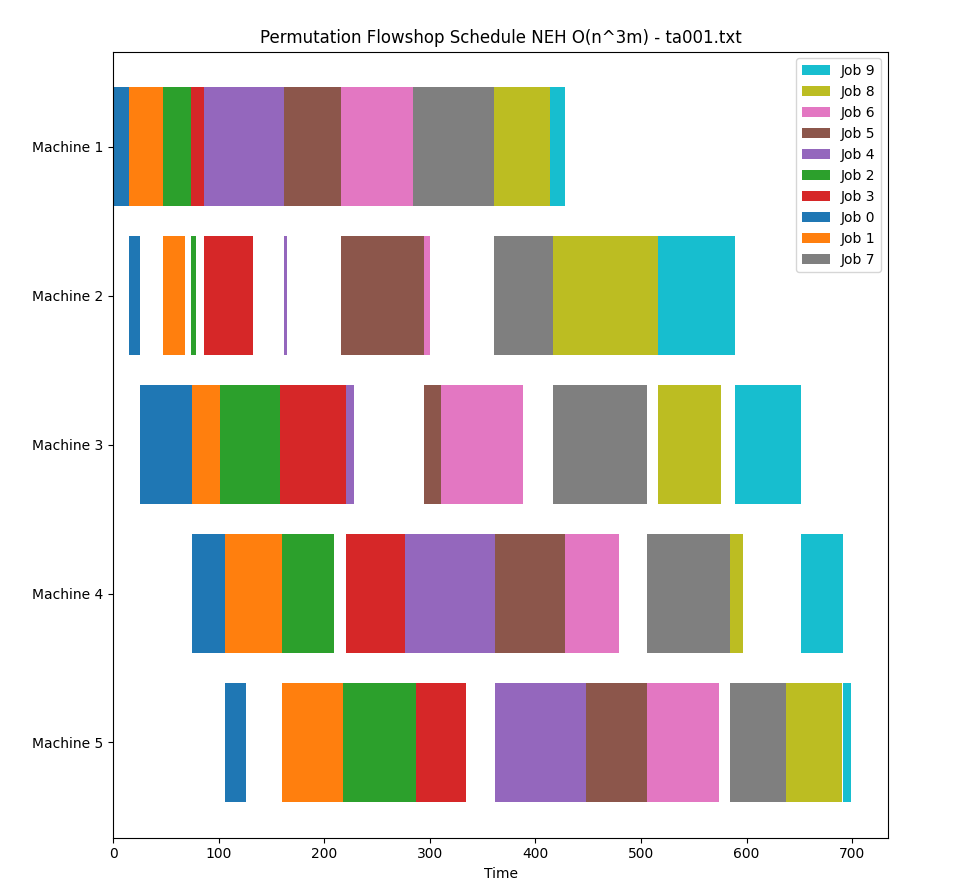
\includegraphics[width=10cm, height=7cm]{neh_run_ta001_gantt.png}
   \caption{Διάγραμμα Gantt του NEH Αλγορίθμου για το αρχείο ta001.txt}
   \label{fig:nehG_ta001}
\end{figure} 

\begin{figure}[H]
   \centering
   \includegraphics[width=10cm, height=7cm]{neh_run_ta020.png}
   \caption{Εκτέλεση NEH Αλγορίθμου για το αρχείο ta020.txt}
   \label{fig:neh_ta020}
\end{figure} 

\begin{figure}[H]
   \centering
   \includegraphics[width=10cm, height=7cm]{neh_run_ta020_gantt.png}
   \caption{Διάγραμμα Gantt του NEH Αλγορίθμου για το αρχείο ta020.txt}
   \label{fig:nehG_ta020}
\end{figure} 


\newpage
\subsection{Απεικόνιση λύσεων προγραμμάτων ως γραφήμματα Gantt}

    Η απεικόνιση των λύσεων προγραμμάτων ως γραφήματα Gantt με το χρόνο στον άξονα x, τις μηχανές στον άξονα y και τις εργασίες ως επιμέρους κουτάκια στις κατάλληλες θέσεις, υλοποιήθηκε με τη χρήση της βιβλιοθήκης \textbf{Matplotlib} στην Python. Η Matplotlib είναι μία από τις πιο δημοφιλείς βιβλιοθήκες γραφικών στην Python και παρέχει ευέλικτα εργαλεία για τη δημιουργία διαγραμμάτων και γραφημάτων.
    Συγκεκριμένα, η χρήση της Matplotlib στον κώδικα περιλαμβάνει την εισαγωγή των εξής μετασχηματιστών: \newline
    \textbf{import matplotlib.pyplot as plt} \\
    \textbf{import matplotlib.colors as mcolors} 

    Με τη χρήση αυτών των βιβλιοθηκών, η συνάρτηση \textbf{\texttt{display\char`_schedule}} δημιουργεί γραφήματα Gantt για την οπτικοποίηση των προγραμμάτων εκτέλεσης των εργασιών, βελτιώνοντας την κατανόηση των αποτελεσμάτων του αλγορίθμου Flowshop Scheduling. Ειδικότερα, η διαδικασία υλοποίησης της απεικόνισης μέσω της \texttt{display\char`_schedule} είναι η εξής:

\begin{enumerate}
   \item \textbf{Δημιουργία Πίνακα Χρόνων Ολοκλήρωσης (\texttt{C\char`_table}):}
   \begin{itemize}
     \item Πριν από την απεικόνιση, υπολογίζεται ο πίνακας χρόνων ολοκλήρωσης \texttt{C\char`_table} για το βέλτιστο πρόγραμμα εκτέλεσης. Αυτός ο πίνακας αποτυπώνει τους χρόνους τερματισμού εκτέλεσης κάθε εργασίας σε κάθε μηχάνημα.
   \end{itemize}
   \item \textbf{Αντιστοίχιση Εργασιών στο Gantt:}
   \begin{itemize}
     \item Η συνάρτηση αντιστοιχίζει κάθε εργασία σε ένα ξεχωριστό χρωματισμένο κουτάκι στο γράφημα Gantt.
     \item Οι εργασίες τοποθετούνται στην κατάλληλη θέση στον άξονα Y (μηχανές) και στην κατάλληλη χρονική στιγμή στον άξονα X, σύμφωνα με τον πίνακα \texttt{C\char`_table}.
   \end{itemize}
   \item \textbf{Χρήση Χρωμάτων για Κάθε Εργασία:}
   \begin{itemize}
     \item Χρησιμοποιούνται διάφορα χρώματα για κάθε εργασία, ώστε να είναι ευανάγνωστο το γράφημα και να διακρίνονται εύκολα οι διάφορες εργασίες..
   \end{itemize}
   \item \textbf{Εμφάνιση Διαγράμματος:}
   \begin{itemize}
     \item Το διάγραμμα Gantt παράγεται με χρήση της βιβλιοθήκης Matplotlib.
     \item Εμφανίζονται τα χρονικά διαστήματα κάθε εργασίας σε κάθε μηχάνημα.
   \end{itemize}
\end{enumerate}

    Έτσι, κατά την εκτέλεση του προγράμματος για κάθε αρχείο εισόδου, προβάλλεται ένα γράφημα Gantt που απεικονίζει το πρόγραμμα εκτέλεσης των εργασιών, καθιστώντας ευανάγνωστο και κατανοητό το αποτέλεσμα του αλγορίθμου Flowshop Scheduling.

\newpage
\subsection{Υλοποίηση βελτιωμένου αλγορίθμου NEH}

    Σύμφωνα με την αναφορά “Some efficient heuristic methods for the flow shop sequencing problem” τα βήματα του NEH αλγορίθμου είναι τα εξής:

\begin{enumerate}
   \item Ταξινόμηση των n εργασιών με βάση τα φθίνοντα αθροίσματα των χρόνων επεξεργασίας στις μηχανές.
   \item Προγραμματισμός των δύο πρώτων εργασιών (schedule) με σκοπό την ελαχιστοποίηση του current makespan σαν να υπήρχαν μόνο αυτές οι δύο εργασίες.
   \item Για k=3 έως n τότε:
   \item Τοποθέτηση της k-οστής εργασίας στη θέση, μεταξύ των k πιθανών, που ελαχιστοποιεί τη μερική διάρκεια (current makespan).
\end{enumerate}

    Όσον αφορά την πολυπλοκότητα σε αυτόν τον αλγόριθμο, στο Βήμα 1 είναι O(n log(n)) και στο Βήμα 2 είναι O(m). Για τον υπολογισμό του current makespan στο Βήμα 4 χρειάστηκαν O(km) πράξεις.

    Εδώ, στο πρόγραμμα nehsquare.py η συγκεκριμένη υλοποίηση επιτυγχάνει τη βελτιστοποίηση του αλγορίθμου NEH, πετυχαίνοντας πολυπλοκότητα O(n\wedge2m). Η κύρια λειτουργία του αλγορίθμου περιγράφεται στη συνάρτηση \texttt{neh\char`_square()}, όπου εκτελείται για κάθε αρχείο εισόδου (πρόβλημα) με τη χρήση της συνάρτησης \texttt{run\char`_neh\char`_square()}. Η αποτελεσματικότητα και η απόδοση του αλγορίθμου αξιολογούνται μέσω της εκτύπωσης των βέλτιστων διατάξεων, των χρόνων εκτέλεσης και άλλων στατιστικών πληροφοριών για κάθε πρόβλημα. Επιπλέον, ο κώδικας παρέχει και τη δυνατότητα οπτικοποίησης της βέλτιστης διάταξης με τη χρήση γραφήματος Gantt μέσω της συνάρτησης \texttt{display\char`_schedule()}, που επισημαίνει την πορεία της κάθε εργασίας σε κάθε μηχάνημα.

    Είναι σημαντικό να τονιστεί όμως, ότι η βελτιωμένη υλοποίηση του NEH αλγορίθμου προσφέρει αξιοσημείωτη απόδοση και αποτελεσματικότητα, καθιστώντας τον αλγόριθμο κατάλληλο για εφαρμογές μεγάλης κλίμακας στον τομέα της χρονοπρογραμματισμού παραγωγικών διεργασιών.
    
    Παρακάτω παρουσιάζονται δύο συγκεκριμένα παραδείγματα εκτέλεσης του κώδικα και των διαγραμμάτων Gantt, για το αρχείο ta001.txt και για το αρχείο ta020.txt :

\begin{figure}[H]
   \centering
   \includegraphics[width=10cm, height=7cm]{neh_square_ta001.png}
   \caption{Εκτέλεση NEH O(n2m)  για το αρχείο ta001.txt}
   \label{fig:square_ta001}
\end{figure} 

\begin{figure}[H]
   \centering
   \includegraphics[width=10cm, height=7cm]{neh_square_gantt_ta001.png}
   \caption{Διάγραμμα Gantt του NEH O(n2m) για το αρχείο ta001.txt}
   \label{fig:squarG_ta001}
\end{figure} 

\begin{figure}[H]
   \centering
   \includegraphics[width=10cm, height=7cm]{neh_square_ta020.png}
   \caption{Εκτέλεση NEH O(n2m)  για το αρχείο ta020.txt}
   \label{fig:squar_ta020}
\end{figure} 

\begin{figure}[H]
   \centering
   \includegraphics[width=10cm, height=7cm]{neh_square_gantt_ta020.png}
   \caption{Διάγραμμα Gantt του NEH O(n2m) για το αρχείο ta020.txt}
   \label{fig:squarG_ta020}
\end{figure} 


\newpage
\subsection{Υλοποίηση διαφορετικής προσέγγισης και σύγκριση αποτελέσμάτων}

    Στην προσέγγισή μου για το πρόβλημα PFSP, επιλέγω να υλοποιήσω τον αλγόριθμο \textbf{Tabu Search}, έναν βελτιωμένο μεταευριστικό (metaheuristic) αλγόριθμο που επιδιώκει την εύρεση βέλτιστων λύσεων σε προβλήματα συνδυαστικής βελτιστοποίησης.
    
    Ο αλγόριθμος Tabu Search λειτουργεί με τη χρήση μιας λίστας "Tabu" που περιέχει κινήσεις που έχουν προσφάτως εξεταστεί, αποφεύγοντας έτσι την επανάληψη των ίδιων κινήσεων. Επιπλέον, χρησιμοποιεί μηχανισμούς όπως η λειτουργία κόστους για την επιλογή βέλτιστων κινήσεων.
    
    Στην πράξη, ο αλγόριθμος Tabu Search ξεκινάει από μια αρχική λύση και εξερευνά διάφορες γειτονικές λύσεις. Οι καλύτερες λύσεις διατηρούνται, ακόμη κι αν αυτές προσθέτουν κινήσεις που βρίσκονται στη λίστα Tabu. Ο αλγόριθμος εξερευνά διάφορες περιοχές του χώρου λύσεων, προσπαθώντας να αποφύγει τον εγκλωβισμό.

\begin{figure}[H]
   \centering
   \includegraphics[width=10cm, height=7cm]{tabu_run_ta001.png}
   \caption{Εκτέλεση Tabu Search  για το αρχείο ta001.txt}
   \label{fig:tabu_ta001}
\end{figure} 

\begin{figure}[H]
   \centering
   \includegraphics[width=10cm, height=7cm]{tabu_run_ta001_gantt.png}
   \caption{Διάγραμμα Gantt του Tabu  για το αρχείο ta001.txt}
   \label{fig:tabu_ta001}
\end{figure}

\begin{figure}[H]
   \centering
   \includegraphics[width=10cm, height=7cm]{tabu_run_ta020.png}
   \caption{Εκτέλεση Tabu Search  για το αρχείο ta020.txt}
   \label{fig:tabu_ta020}
\end{figure} 

\begin{figure}[H]
   \centering
   \includegraphics[width=10cm, height=7cm]{tabu_run_ta020_gantt.png}
   \caption{Διάγραμμα Gantt του Tabu  για το αρχείο ta020.txt}
   \label{fig:tabu_ta001}
\end{figure}
    
    Για τη σύγκριση των αποτελεσμάτων του Tabu Search με αυτά του NEH, εκτελώ τους δύο αλγορίθμους για τα ίδια προβλήματα PFSP και αξιολογώ την απόδοσή τους βάσει του makespan. Προσέγγιση του ποιοτικού και ποσοτικού κριτηρίου των λύσεων μεταξύ των δύο αλγορίθμων θα με διαφωτίσει σχετικά με την αποτελεσματικότητά τους για το συγκεκριμένο πρόβλημα. Εδώ, χρησιμοποιήθηκε το Matlab για πιο λεπτομερής ανάλυση των αποτελεσμάτων στα γραφήματα. Τα δεδομένα για το makespan του NEH αλγορίθμου, καθώς και εκείνα του Tabu Αλγορίθμου, αποθηκευόταν αυτόματα κατά την εκτέλεση του κάθε κώδικα αντίστοιχα σε ένα αρχείο με το όνομα \texttt{makespan\char`_neh\char`_algorithm.txt} και \texttt{makespan\char`_tabu\char`_algorithm.txt} αντίστοιχα. Ο κώδικας είναι ο εξής:

\begin{figure}[H]
   \centering
   \includegraphics[width=10cm, height=7cm]{matlab.png}
   \caption{Ο κώδικας σύγκρισης NEH με Tabu Αλγόριθμο σε MATLAB}
   \label{fig:matlabcode}
\end{figure} 

\begin{figure}[H]
   \centering
   \includegraphics[width=10cm, height=7cm]{neh_vs_tabu.png}
   \caption{Σύγκριση των Makespans του NEH με του Tabu Search}
   \label{fig:matlabplot}
\end{figure} 

\newpage
\section{Εκτέλεση Αρχείων}

    Η εκτέλεση της υλοποίησης των αλγορίθμων για την επίλυση του προβλήματος PFSP πραγματοποιήθηκε με χρήση της γλώσσας προγραμματισμού Python. Πριν από την εκτέλεση των αλγορίθμων, οι χρήστες πρέπει να σιγουρευτούν ότι έχετε εγκαταστήσει όλες τις απαιτούμενες βιβλιοθήκες Python που χρησιμοποιούνται στον κώδικα, χρησιμοποιώντας τον διαχειριστή πακέτων της Python (π.χ. pip).
    Οι χρήστες μπορούν να εκτελέσουν τον κώδικα μέσω του τερματικού (Command Window) ή του περιβάλλοντος εκτέλεσης Python. Είναι σημαντικό να παρέχουν τις κατάλληλες παραμέτρους και διαδρομές αρχείων, όπως η τοποθεσία των στιγμιοτύπων των προβλημάτων PFSP. Πιο συγκεκριμένα:

\begin{itemize}
  \item \textbf{Εκτέλεση \texttt{neh\char`_algorithm.py}:} python \texttt{neh\char`_algorithm.py}
  \item \textbf{Εκτέλεση \texttt{neh\char`_square.py}:} python \texttt{neh\char`_square.py}
  \item \textbf{Εκτέλεση \texttt{tabu\char`_algorithm.py}:} python \texttt{tabu\char`_algorithm.py}
\end{itemize}

    Ακόμη, όλα τα αρχεία της συγκεκριμένης εργασίας είναι ανεβασμένα στο public repository στο GitHub : \url{https://github.com/penyvinni/AADS_PFSP_170}. Η διαδικασία που ακολουθήθηκε είναι η εξής:
    
\begin{itemize}
  \item Δημιουργία Νέου Αποθετηρίου (Repository) στο GitHub
  \item Προετοιμασία του Τοπικού Αποθετηρίου (Local Repository) μέσω του Git Bash.
  \item Εκτέλεση των εντολών: 
  \begin{itemize}
     \item git init
     \item git add .
     \item git commit -m "First Commit" 
  \end{itemize}
  \item Σύνδεση του Τοπικού με το Κοινόχρηστο Αποθετήριο με την εντολή:
   \begin{itemize}
     \item git remote add origin \texttt{<repository\char`_ur>}
  \end{itemize}
  \item Ανέβασμα των Αλλαγών στο GitHub με την εντολή :
     \begin{itemize}
     \item git push -u origin master 
  \end{itemize}
\end{itemize}


\newpage
\section{Συμπεράσματα}

    Συμπερασματικά, στο πλαίσιο της συγκεκριμένης εργασίας, προσφέρθηκε μια εκτενής μελέτη επίλυσης του PFSP, εξετάζοντας διάφορες προσεγγίσεις. Αρχικά, προσεγγίθηκε το πρόβλημα με τον ευρετικό αλγόριθμο NEH, αποτυπώνοντας τις λύσεις μέσω γραφημάτων Gantt για καλύτερη κατανόηση. Εν συνεχεία, υλοποιήθηκε ή βελτίωση του αλγορίθμου όπως προτείνεται στη βιβλιογραφία, μειώνοντας σημαντικά την πολυπλοκότητά του. Η ανάλυση χρόνων εκτέλεσης κατέδειξε την αποτελεσματικότητα της βελτιωμένης προσέγγισης.
    
    Επιπλέον, έγινε πρόταση μια προσωπικής προσέγγισης για την επίλυση του προβλήματος, η οποία συγκρίθηκε με τα αποτελέσματα του NEH. Η σύγκριση αυτή αποκάλυψε τα πλεονεκτήματα και τα χαρακτηριστικά κάθε προσεγγίσεως, ενισχύοντας την κατανόηση των δυνατοτήτων και των περιορισμών των αλγορίθμων που εξετάστηκαν. Η προσέγγιση αυτή συμβάλλει στην εμβάθυνση της γνώσης μας σχετικά με τις προκλήσεις του PFSP και ενισχύει την ευελιξία του αναλυτικού πλαισίου για παρόμοια προβλήματα χρονοπρογραμματισμού στο μέλλον.
 

\end{document}